\documentclass[12pt]{scrartcl}
\usepackage[sexy]{evan}
\usepackage{graphicx,amsmath,amssymb,amsthm,amsfonts,babel}
\usepackage{tikz, tkz-euclide}
\usepackage{lipsum}
\usepackage{setspace}
\graphicspath{ {./} }
\usetikzlibrary{calc,through,intersections}
%\usepackage[paperwidth=16cm, paperheight=16cm,margin=1cm]{geometry}

\colorlet{EvanRed}{Red!50!Purple}
\definecolor{officegreen}{rgb}{0.0, 0.5, 0.0}

\newcommand{\siku}[4][.2cm]
	{
	\coordinate (tempa) at ($(#3)!#1!(#2)$);
	\coordinate (tempb) at ($(#3)!#1!(#4)$);
	\coordinate (tempc) at ($(tempa)!0.5!(tempb)$);%midpoint
	\draw[black] (tempa) -- ($(#3)!2!(tempc)$) -- (tempb);
	}
	\usetikzlibrary{calc,positioning,intersections}

\setstretch{1.5}

\usepackage{etoolbox}
\newcommand{\zerodisplayskips}{%
  \setlength{\abovedisplayskip}{5pt}%
  \setlength{\belowdisplayskip}{5pt}%
  \setlength{\abovedisplayshortskip}{5pt}%
  \setlength{\belowdisplayshortskip}{5pt}}
\appto{\normalsize}{\zerodisplayskips}
\appto{\small}{\zerodisplayskips}
\appto{\footnotesize}{\zerodisplayskips}
\setlength\parindent{10pt}

\title{Solusi OSN-K Matematika SMA 2023}
\author{Azzam Labib Hakim}
\date{last update: \today}


\begin{document}
\maketitle
%\pagestyle{plain}
\vspace{-1.5cm}
\section{Soal}
\subsection{Kemampuan Dasar}
\begin{enumerate}
\item Hasil penjumlahan semua solusi persamaan
\begin{align*}
|x-|2x+6||=99
\end{align*}
adalah \dots

\item Di dalam suatu laci terdapat 7 pasang kaos kaki yang setiap pasangnya berbeda dengan pasangan lain. Diambil 6 kaos kaki sekaligus secara acak. Banyak cara pengambilan sehingga diantara yang terambil terdapat \textbf{tepat} sepasang kaos kaki yang berpasangan adalah \dots

\item Diberikan trapesium $ABCD$ dengan $AB = 13$, $CD = 18$, $AB$ sejajar $CD$,
dan $\angle ADC$, $\angle BCD$ keduanya dibawah $90^\circ$. Jika $P$ dan $Q$ adalah titik pada sisi $CD$ sehingga $AD = AP$ dan $BC = BQ$, tentukan nilai dari $PQ$.

\item Suatu bilangan empat digit $8ab9$ merupakan suatu bilangan kuadrat. Nilai dari $a+b$ adalah \dots

\item Diberikan fungsi kuadrat  $f(x) = ax^2+bx+c$ yang memenuhi $f(4)=16$ dan $f(7)=49$. Jika $a \neq 1$, nilai dari $\frac{c-b}{a-1}$ adalah \dots

\item Dua tim $A$ dan $B$ bertanding sepak bola sebanyak 13 kali. Tiap pertandingan, tim yang berhasil mencetak 5 gol pertama adalah pemenang dan tidak ada pertandingan yang berakhir seri. Selama 13 pertandingan, tim $A$ menang lebih banyak dari $B$, sedangkan gol tim $B$ lebih banyak dari tim $A$. Selisih total gol terbesar antara kedua tim tersebut adalah \dots

\item Diberikan segitiga lancip $ABC$ dengan panjang $AB = 12$ dan $AC = 10$. $D$ adalah suatu titik di $BC$. $E$ dan $F$ adalah titik berat segitiga $ABD$ dan $ACD$ berturut-turut. Jika luas dari segitiga $DEF$ sama dengan 4, dan panjang $BC = \sqrt{n}$, tentukan nilai dari $n$.

\item Sisa pembagian dari $5^{2021}+11^{2022}$ oleh 64 adalah \dots

\item Diberikan suku banyak dengan koefisien bilangan bulat $P(x)$. Jika
$$P(r_1)=P(r_2)=220$$
dengan $r_1$ dan $r_2$ merupakan akar-akar dari persamaan kuadrat $x^2+x-25=0$. Maka, sisa pembagian $P(1)$ oleh $23$ adalah \dots

\item Banyak bilangan 4 digit yang habis dibagi 3 dan memuat angka 6 adalah \dots
\end{enumerate}

\newpage
\subsection{Kemampuan Lanjut}
\begin{enumerate}[resume]
\item Diberikan segiempat $ABCD$ siklis dengan lingkaran luarnya adalah $\omega$. Panjang $BC=CD$, $AC$ memotong $BD$ di titik $E$, $BE=7$, dan $DE=4$. Garis singgung $\omega$ di titik $A$ memotong $BD$ di titik $P$. Jika $\frac{PD}{PB}$ dapat ditulis dalam bentuk $\frac{m}{n}$ dengan $m$ dan $n$ adalah bilangan asli yang saling relatif prima, tentukan nilai dari $m+n$.

\item Jika bilangan asli $x$ dan $y$ memenuhi
$$x(x-y)=6y-7,$$
nilai dari $x+y$ adalah \dots

\item Misalkan $a_1,a_2,a_3,\dots$ suatu barisan yang memenuhi persamaan
$$a_{n+2}-a_{n+1}+a_{n}=\dfrac{n+2}{6}$$
untuk setiap bilangan asli $n$. Jika $a_1=3$ dan $a_2=4$, tentukan nilai dari $a_{2023}$.

\item Diberikan himpunan $S = \{a,b,c,d,e,f\}$. Akan dipilih dua subhimpunan dari $S$ yang gabungannya adalah $S$. Subhimpunan yang dipilih tidak harus berbeda. Urutan dari subhimpunan tidak diperhatikan. Banyak cara melakukan pemilihan adalah \dots

\item Diberikan lingkaran $\Omega$ dan $AB$ merupakan tali busur dari $\Omega$. Lingkaran $\omega_1$ menyinggung $\Omega$ secara internal dan menyinggung $AB$ pada titik tengahnya. Lingkaran $\omega_2$ menyinggung $\Omega$ secara internal dan $\omega_1$ secara eksternal serta menyinggung $AB$. Jika jari-jari dari $\omega_1$ adalah 40 dan jari-jari dari $\omega_2$ adalah 8, tentukan panjang dari $AB$.
\begin{center}
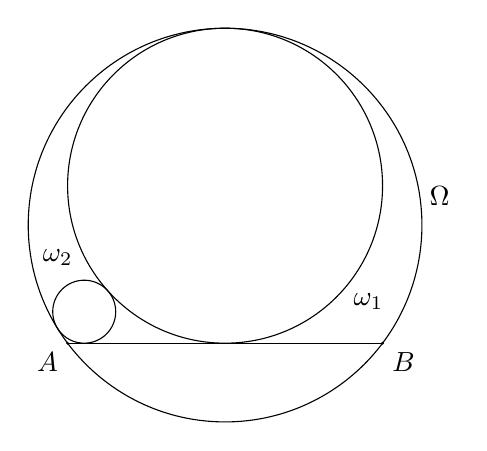
\begin{tikzpicture}[scale=0.5]
% draw circles
\coordinate (O) at (0,0);
\draw (O) circle [radius=5cm] node[label={$\Omega$}, right=2.6cm] {};
\coordinate (C) at (0,1);
\draw (C) circle [radius=4cm] node[label={$\omega_1$}, below right=2.4cm] {};
\coordinate (D) at (-3.57771, -2.2);
\draw (D) circle [radius=0.8cm] node[label={$\omega_2$}, above left=0.3cm] {};
% segment AB
\coordinate[label=below left:$A$] (A) at (-4,-3);
\fill (A) circle (0.04cm);
\coordinate[label=below right:$B$] (B) at (4,-3);
\fill (B) circle (0.04cm);
% segment
\draw (A) -- (B);
\end{tikzpicture}
\end{center}

\item Misal, $N = 2^a \cdot 3^b$ dengan $a, b$ bilangan asli. Jika hasil kali semua faktor positif dari $N$ adalah $24^{60}$, maka nilai $ab$ adalah \dots

\item Nilai minimum dari
$$\dfrac{(x+y)^2}{\sqrt{x^2-9}+\sqrt{y^2-16}}$$
adalah \dots

\item Diberikan 100 titik seperti pada gambar berikut (jarak tiap titik sama)
\begin{center}
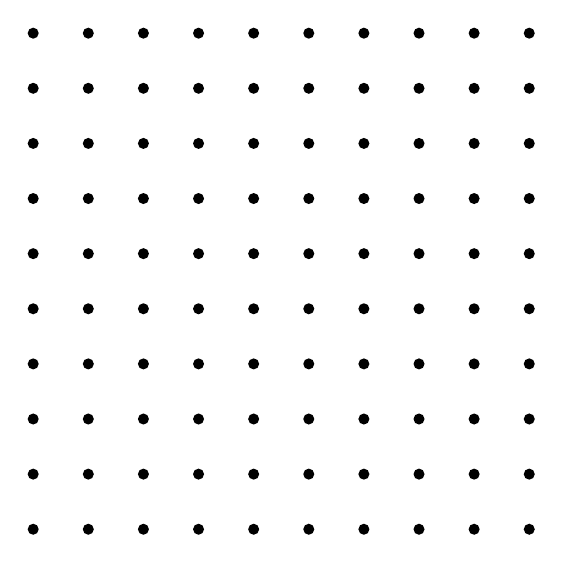
\begin{tikzpicture}[scale=0.7]
    \draw[step=1cm,draw opacity=0.0] (0,0) grid (9,9);
    \foreach \x in {0,1,2,...,9}
        \foreach \y in {0,1,2,...,9}
            \fill (\x,\y) circle (0.1cm);
\end{tikzpicture}
\end{center}
Banyak persegi yang semua titik sudutnya adalah 4 titik diantara titik-titik pada gambar tersebut adalah \dots

\item Diberikan segitiga $ABC$. Misal titik $D,E,F$ terletak pada sisi $BC,CA,AB$ sehingga $AD,BE,CF$ berpotongan di satu titik. Diketahui bahwa $\angle EDF = 56^\circ$. Jika $\angle ADB = 90^\circ$ dan $AF=FB$, maka besar sudut $\angle ABC$ adalah \dots

\item Misal $p$ dan $n$ adalah dua bilangan asli dengan $p$ prima sehingga $p$ membagi $n^2+4$ dan $n$ membagi $p^2+4$. Jika $p<200$, nilai terbesar yang mungkin dari $n$ adalah \dots
\end{enumerate}

\newpage
\section{Solusi}
\subsection{Kemampuan Dasar}
\begin{soalbaru}
Hasil penjumlahan semua solusi persamaan
\begin{align*}
|x-|2x+6||=99
\end{align*}
adalah \dots
\end{soalbaru}
\begin{jawaban}
58
\end{jawaban}
\begin{solusi}
Bagi kasus untuk $x \ge -\tfrac{6}{2}$ atau $x < -\tfrac{6}{2}$.

Jika $x \ge -\tfrac{6}{2}$, maka $|2x+6| = 2x+6$. Jelas bahwa $x > -6$ sehingga $|x+6|=x+6$ yang mana
$$99=|x-|2x+6||=|x-(2x+6)|=|-x-6|=|x+6|=x+6 \implies x = 93.$$

Jika $x < -\tfrac{6}{2}$, maka $|2x+6| = -2x-6$. Maka
$$99=|x-|2x+6||=|x-(-2x-6)|=|3x+6|=3|x+6| \implies 33=|x+2|.$$
Akan dibagi kasus lagi:
\begin{itemize}
\item Jika $x \ge -2$ sehingga $|x+2|=x+2$ maka $33=x+2 \implies x=31$. Solusi ini tidak memenuhi karena harusnya $-2 \le x < -\tfrac{6}{2}$.
\item Jika $x < -2$ sehingga $|x+2|=-(x+2)$ maka $33=-x-2 \implies x=-35$.
\end{itemize}
Cek semua solusi diatas, hanya $x=93$ dan $x=-35$ yang memenuhi. Berarti hasil penjumlahan semua solusinya adalah $93+(-35)=\boxed{58}$.

\end{solusi}

\begin{soalbaru}
Di dalam suatu laci terdapat 7 pasang kaos kaki yang setiap pasangnya berbeda dengan pasangan lain. Diambil 6 kaos kaki sekaligus secara acak. Banyak cara pengambilan sehingga diantara yang terambil terdapat \textbf{tepat} sepasang kaos kaki yang berpasangan adalah \dots
\end{soalbaru}
\begin{jawaban}
105
\end{jawaban}
\begin{solusi}
\textbf{Asumsi kaus kaki kiri dan kanan identik}: Pertama ambil 5 buah kaus kaki berbeda dari masing-masing pasangan yang ada, berarti ada ${7 \choose 5} = 21$ kemungkinan berbeda. Lalu, diambil 1 kaus kaki lagi dari $2 \times 7 - 5 = 9$ kaus kaki tersisa sehingga dapat dipasangkan dengan salah satu 5 kaus kaki yang tadi sudah terambil. Karena awalnya setiap kaus kaki berpasangan, dapat dipastikan kita dapat mengambil salah satu dari 5 kaus kaki untuk dipasangkan, sehingga ada ${5 \choose 1}=5$ kemungkinan. Berarti total banyak cara pengambilan yang mungkin adalah $21 \times 5 = \boxed{105}$.\\
\textbf{Asumsi kaus kaki kiri dan kanan berbeda}: Mirip dengan cara sebelumnya, hanya saja keempat kaus kaki terpilih yang tidak berpasangan masing-masing mempunyai 2 kemungkinan yaitu kiri dan kanan, sehingga banyak cara pengambilan sebelumnya dikalikan dengan $2^4 = 16$ sehingga banyak cara pengambilan total menjadi $105 \cdot 16 = \boxed{1680}$.
\end{solusi}

\begin{soalbaru}
Diberikan trapesium $ABCD$ dengan $AB = 13$, $CD = 18$, $AB$ sejajar $CD$,
dan $\angle ADC$, $\angle BCD$ keduanya dibawah $90^\circ$. Jika $P$ dan $Q$ adalah titik pada sisi $CD$ sehingga $AD = AP$ dan $BC = BQ$, tentukan nilai dari $PQ$.
\end{soalbaru}
\begin{jawaban}
8
\end{jawaban}
\begin{solusi}
Misalkan $M$ dan $N$ berturut-turut merupakan proyeksi titik $A$ dan $B$ pada garis $BC$. 
\begin{center}
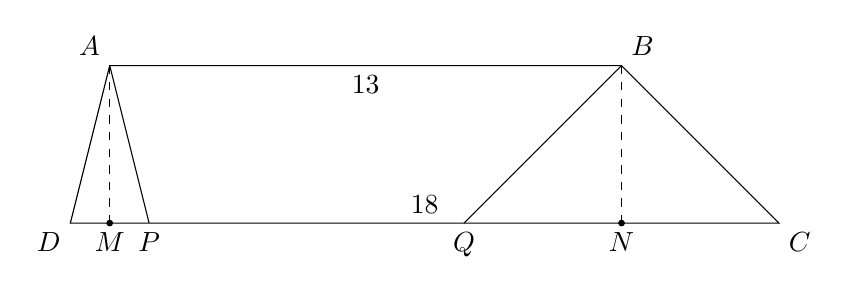
\begin{tikzpicture}[scale=0.5]
% define points A, B, C, D
\coordinate[label=below left:$D$] (D) at (0,0);
\coordinate[label=below right:$C$] (C) at (18,0);
\coordinate[label=above right:$B$] (B) at (14,4);
\coordinate[label=above left:$A$] (A) at (1,4);
% draw trapezoid
\draw (A) -- (B) -- (C) -- (D) -- cycle;
% add points M and N
\coordinate[label=below:$M$] (M) at ($(C)!(A)!(D)$);
\coordinate[label=below:$N$] (N) at ($(C)!(B)!(D)$);
\filldraw (M) circle (2pt);
\filldraw (N) circle (2pt);
% draw perpendicular line and label
\draw[dashed] (A) -- (M);
\draw[dashed] (B) -- (N);
% draw P and Q
\coordinate[label=below:$P$] (P) at ($(M)!-1!(D)$);
\coordinate[label=below:$Q$] (Q) at ($(N)!-1!(C)$);
% draw AP and BQ
\draw (A) -- (P);
\draw (B) -- (Q);
% label the sides
\node at ($(A)!0.5!(B)$) [below] {13};
\node at ($(C)!0.5!(D)$) [above] {18};
\end{tikzpicture}
\end{center}
Berarti karena $AM, BN \perp BC \parallel CD$, $AD=AP$ dan $BQ=BC$ maka $DM=MP$ dan $QN=NC$. Di lain sisi, karena $ABNM$ adalah persegi panjang, maka $MN=AB=13$. Berarti $DM+NC=DC-MN=18-13=5$. Hal ini mengakibatkan 
\begin{align*}
PQ &= DC-(DM+MP+QN+NC)\\
&= DC - (DM+DM+NC+NC)\\
&= DC-2(DM+NC)\\
&= 18 - 2(5)\\
&= \boxed{8}.
\end{align*}
\end{solusi}

\begin{soalbaru}
Suatu bilangan empat digit $8ab9$ merupakan suatu bilangan kuadrat. Nilai dari $a+b$ adalah \dots
\end{soalbaru}
\begin{jawaban}
10
\end{jawaban}
\begin{solusi}
Perhatikan bahwa $89^2 = 7921 < \overline{8ab9} < 10000 = 100^2$. Berarti dapat dimisalkan $\overline{8ab9} = \overline{9x}^2$ dimana $x \in \{0,1,2,\dots, 9\}$. Karena digit terakhir dari $\overline{9x}^2$ adalah 9, maka $x$ yang mungkin adalah $3$ atau $7$. Namun, jika $x = 7$, maka $\overline{9x}^2 = 97^2 = 9409 > \overline{8ab9}$, kontradiksi. Oleh karena itu, haruslah $x=3$ sehingga $\overline{8ab9}=\overline{9x}^2 = 93^2 = 8649$ yang menyebabkan $a=6$ dan $b=4$. Diperoleh $a+b = \boxed{10}$.
\end{solusi}

\begin{soalbaru}
Diberikan fungsi kuadrat  $f(x) = ax^2+bx+c$ yang memenuhi $f(4)=16$ dan $f(7)=49$. Jika $a \neq 1$, nilai dari $\frac{c-b}{a-1}$ adalah \dots
\end{soalbaru}
\begin{jawaban}
39
\end{jawaban}
\begin{solusi}
Kita punya $f(4)=16a+4b+c=16$ dan $f(7)=49a+7b+c=49$. Berarti 
\begin{align*}
(49a+7b+c)-(16a+4b+c)&=49-16\\
33a+3b &= 33\\
11a+b &= 11\\
b &= -11(a-1)
\end{align*}
Di lain sisi
\begin{align*}
16a+4b+c&=16\\
16(a-1) + 4b + c &= 0\\
-\frac{16}{11}b + 4b + c &= 0\\
c &= -\frac{28}{11}b
\end{align*}
Itu berarti 
\begin{align*}
\dfrac{c-b}{a-1} = \dfrac{-\frac{28}{11}b-b}{-\frac{b}{11}}=\boxed{39}.
\end{align*}
\end{solusi}

\begin{soalbaru}
Dua tim $A$ dan $B$ bertanding sepak bola sebanyak 13 kali. Tiap pertandingan, tim yang berhasil mencetak 5 gol pertama adalah pemenang dan tidak ada pertandingan yang berakhir seri. Selama 13 pertandingan, tim $A$ menang lebih banyak dari $B$, sedangkan gol tim $B$ lebih banyak dari tim $A$. Selisih total gol terbesar antara kedua tim tersebut adalah \dots
\end{soalbaru}
\begin{jawaban}
23
\end{jawaban}
\begin{solusi}
Misalkan tim $A$ menang $x$ kali dan tim $B$ menang $y$ kali dengan $x+y=13$ dan $x>y$. Maka $x \ge 7$ dan $y  \le 6$. Perhatikan agar selisih gol antara $B$ dan $A$ sebesar mungkin maka $B$ harus mendapatkan gol sebesar mungkin di setiap pertandingan dan $A$ harus mendapatkan gol sesedikit mungkin di setiap pertandingan. Tim $B$ harus mendapatkan $4$ gol di setiap pertandingan yang dimenangkan tim $A$ dimana tim $A$ mendapatkan 5 gol dan di lain pihak tim $B$ mendapatkan $5$ gol di setiap pertandingan yang dimenangkan tim $B$ dengan tim $A$ harus mendapatkan $0$ gol. Oleh karena itu, total gol yang didapatkan tim $A$ adalah $5x+0$ dan total gol yang didapatkan tim $B$ adalah $5y+4x$. Itu berarti selisih gol antara kedua tim adalah
$$(5y+4x)-(5x+0) = 5y-x = 5y - (13-y) = 6y - 13 \le 6 \cdot 6 - 13 = \boxed{23}$$
dengan kesamaan (maksimum) terjadi saat $y=6$.
\end{solusi}

\begin{soalbaru}
Diberikan segitiga lancip $ABC$ dengan panjang $AB = 12$ dan $AC = 10$. $D$ adalah suatu titik di $BC$. $E$ dan $F$ adalah titik berat segitiga $ABD$ dan $ACD$ berturut-turut. Jika luas dari segitiga $DEF$ sama dengan 4, dan panjang $BC = \sqrt{n}$, tentukan nilai dari $n$.
\end{soalbaru}
\begin{jawaban}
52
\end{jawaban}
\begin{solusi}
Misalkan $DE$ memotong $AB$ di $K$ dan $DF$ memotong $AC$ di $L$. Dari definisi $E$ dan $F$ sebagai titik berat, didapat bahwa $K$ dan $L$ berturut-turut adalah titik tengah dari $AB$ dan $AC$. 
\begin{center}
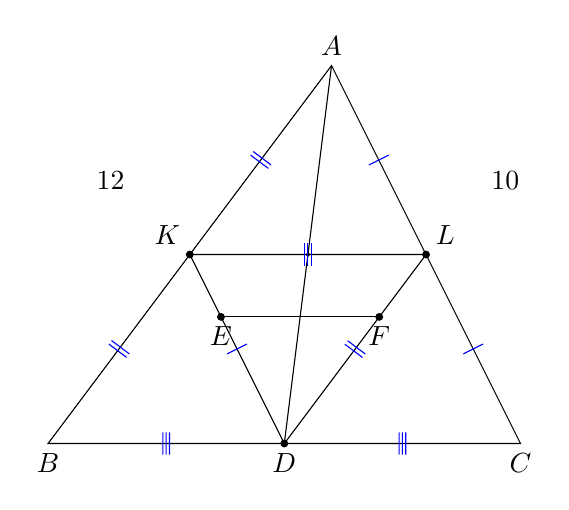
\begin{tikzpicture}[scale=0.6]
% define points A, B, C
\coordinate[label=above:$A$] (A) at (0,0);
\coordinate[label=below:$B$] (B) at (-6,-8);
\coordinate[label=below:$C$] (C) at (4,-8);
% calculate midpoints
\coordinate[label=above left:$K$] (K) at ($(A)!0.5!(B)$);
\coordinate[label=above right:$L$] (L) at ($(A)!0.5!(C)$);
\coordinate[label=below:$D$] (D) at ($(B)!0.5!(C)$);
% draw triangle and midpoints
\draw (A) -- (B) -- (C) -- cycle;
\filldraw (K) circle (2pt);
\filldraw (L) circle (2pt);
\filldraw (D) circle (2pt);
% label sides
\node[above left=10mm] at ($(A)!0.5!(B)$) {12};
\node[above right=10mm] at ($(A)!0.5!(C)$) {10};
\draw (D)--(K)--(L)--cycle;
% E and F
\coordinate[label=below:$E$] (E) at ($(K)!0.33!(D)$);
\coordinate[label=below:$F$] (F) at ($(L)!0.33!(D)$);
\filldraw (E) circle (2pt);
\filldraw (F) circle (2pt);
\draw (E) -- (F);
\draw (A) -- (D);
\filldraw ($(K)!0.5!(L)$) circle (1pt);
% mark same  length segment
\tkzMarkSegment[color=blue,pos=.5,mark=||](A,K) 
\tkzMarkSegment[color=blue,pos=.5,mark=||](K,B)
\tkzMarkSegment[color=blue,pos=.5,mark=||](D,L)
\tkzMarkSegment[color=blue,pos=.5,mark=|](A,L) 
\tkzMarkSegment[color=blue,pos=.5,mark=|](L,C)
\tkzMarkSegment[color=blue,pos=.5,mark=|](K,D)
\tkzMarkSegment[color=blue,pos=.5,mark=|||](B,D) 
\tkzMarkSegment[color=blue,pos=.5,mark=|||](D,C) 
\tkzMarkSegment[color=blue,pos=.5,mark=|||](K,L) 
\end{tikzpicture}
\end{center}
Perhatikan karena $E$ titik berat $\triangle ABD$, maka $DE:DK = 2:3$. Karena $F$ titik berat $\triangle ADC$, maka $DF:FL=2:3$. Berarti diperoleh $\triangle EDF \sim \triangle KDL$ sehingga 
$$\dfrac{[EDF]}{[KDL]} = \dfrac{DE^2}{DK^2} = \dfrac{2^2}{3^2}=\dfrac{4}{9} \implies [KDL] = \dfrac{9}{4}[EDF] = 9.$$

Selanjutnya, karena $AK:AB=AL:AC=1:2$ maka $\triangle AKL \sim \triangle ABC$ dengan $KL=\frac{1}{2}BC$. Dengan cara serupa diperoleh juga bahwa $DK=\frac{1}{2}AC$ dan $DL=\frac{1}{2}AB$. Hal ini menyebabkan $\triangle DKL \sim \triangle ACB$ dan $\triangle DKL \cong \triangle ALK$. Berarti 
$$\dfrac{[KDL]}{[ABC]}=\dfrac{[AKL]}{[ABC]}=\dfrac{AK^2}{AB^2}=\dfrac{1^2}{2^2}=\dfrac{1}{4} \implies [ABC] = 4[KDL] = 36.$$

Sekarang, dengan rumus luas sinus kita punya
$$[ABC] = \dfrac{1}{2}\cdot AB \cdot AC \cdot \sin \angle BAC \implies 36=\dfrac{1}{2}\cdot 12 \cdot 10 \cdot \sin \angle BAC \implies \sin \angle BAC = \dfrac{3}{5}.$$
Lalu, karena $\angle BAC < 90^\circ$ maka $\cos \angle BAC = \sqrt{1-\sin^2 \angle BAC} = \sqrt{1 - (\frac{3}{5})^2} = \frac{4}{5}$. Oleh karena itu, dengan dalil cosinus pada $\triangle ABC$ didapat
\begin{align*}
BC^2 &= AB^2 + AC^2 -2\cdot AB \cdot AC \cdot \cos \angle BAC\\
n &= 12^2+10^2 - 2 \cdot 12 \cdot 10 \cdot \frac{4}{5}\\
n &= \boxed{52}.
\end{align*}
\end{solusi}

\begin{soalbaru}
Sisa pembagian dari $5^{2021}+11^{2022}$ oleh 64 adalah \dots
\end{soalbaru}
\begin{jawaban}
30
\end{jawaban}
\begin{solusi}
Perhatikan karena $5$ dan $11$ relatif prima dengan $64$ dan nilai $\phi(64) = 64(1-\frac{1}{2})=32$, maka dengan teorema Euler, $5^{32} \equiv 1 \mod 64$ dan $11^{32} \equiv 1 \mod 64$. Oleh karena itu
$$5^{2021} \equiv (5^{32})^{63} \cdot 5^5 \equiv 1^{63} \cdot 3125 \equiv 53 \mod 64$$
dan karena $11^2 \equiv 121 \equiv -7 \mod 64$ maka
$$11^{2022} \equiv (11^{32})^{63} \cdot (11^2)^3 \equiv 1^{63} \cdot (-7)^3 \equiv -343 \equiv 41 \mod 64$$
Maka didapat $5^{2021}+11^{2022} \equiv 53+41 \equiv 94 \equiv \boxed{30} \mod 64$.
\end{solusi}

\begin{soalbaru}
Diberikan suku banyak dengan koefisien bilangan bulat $P(x)$. Jika
$$P(r_1)=P(r_2)=220$$
dengan $r_1$ dan $r_2$ merupakan akar-akar dari persamaan kuadrat $x^2+x-25=0$. Maka, sisa pembagian $P(1)$ oleh $23$ adalah \dots
\end{soalbaru}
\begin{jawaban}
13
\end{jawaban}
\begin{solusi}
Perhatikan bahwa $x^2+x-25=(x-r_1)(x-r_2)$ dengan $r_1 \neq r_2$. Misalkan $Q(x) = P(x) - 220$ dengan $Q$ adalah suatu polinomial dengan derajat yang sama dengan derajat $P$. Tinjau bahwa $Q(r_1)=Q(r_2)=0$. Dari sini dapat ditulis
$$Q(x)=(x-r_1)(x-r_2)R(x)=(x^2+x-25)R(x)$$
untuk suatu polinomial $R$ dengan $\operatorname{deg}(R) = \operatorname{deg}(P)-2$. Oleh karena itu
$$P(x)=(x^2+x-25)R(x)+220$$ 
sehingga $$P(1) = (1^2+1-25)R(1) + 220 = -23R(1) + 220 \equiv 0 + 13 \equiv \boxed{13} \mod 23.$$
\end{solusi}

\begin{soalbaru}
Banyak bilangan 4 digit yang habis dibagi 3 dan memuat angka 6 adalah \dots
\end{soalbaru}
\begin{jawaban}
1056
\end{jawaban}
\begin{solusi}
Perhatikan bahwa seluruh bilangan 4 digit yang habis dibagi 3 (tanpa syarat lain) dari 1000 sampai 9999 ada sebanyak $\frac{9999-999}{3}=3000$. 

Selanjutnya, akan dihitung banyaknya bilangan 4 digit yang habis dibagi 3 dan tidak memuat angka 6. Misalkan $T = \{0,1,2,3,4,5,7,8,9\}$. 

Pertama akan ditinjau dulu semua bilangan 4 digit yang tidak memuat angka 6, sebut bilangan ini sebagai $x$. Kemungkinan digit pertama bilangan ini adalah $T - \{0\}$, sehingga ada sebanyak $8$ kemungkinan. Lalu, untuk digit kedua, ketiga, dan keempat bilangan ini masing-masing adalah anggota dari $T$ sehingga banyak kemungkinan masing-masing digit tersebut adalah 8. Oleh karena itu, banyaknya $x$ yang mungkin adalah $8 \cdot 9 \cdot 9 \cdot 9$.

Sekarang misalkan $y = \overline{abcd}$ adalah bilangan 4 digit yang tidak memuat angka 6 dan habis dibagi 3. Perhatikan bahwa digit pertama, kedua, dan ketiga dari $y$ tidak mungkin 6. Lalu, tinjau satu-satu nilai yang mungkin bagi $d$. Tinjau setiap himpunan 
\begin{align*}
Y_1 &=\{\overline{abc0},\overline{abc1},\overline{abc2}\}\\ 
Y_2 &=\{\overline{abc3},\overline{abc4},\overline{abc5}\}\\
Y_3 &=\{\overline{abc7},\overline{abc8},\overline{abc9}\}
\end{align*}
Dikarenakan setiap himpunan $Y_i$ berisi 3 bilangan asli berurutan, pasti terdapat tepat satu bilangan yang habis dibagi 3. Oleh karena itu, ada tepat satu bilangan yang habis dibagi oleh 3 pada masing-masing himpunan $Y_1,Y_2,Y_3$. Oleh karena untuk setiap $a,b,c$ yang memenuhi, kita punya $|Y_1|=|Y_2|=|Y_3|$, sehingga menurut konsep kesimetrian, dari seluruh bilangan $x$ yang mungkin, $\frac{1}{3}$ nya adalah bilangan $y$. Oleh karena itu, banyaknya $y$ yang mungkin adalah $\frac{1}{3}\cdot 8 \cdot 9 \cdot 9 \cdot 9 = 1944$.

Dari fakta-fakta tersebut, dengan konsep komplemen (inklusi-eksklusi), banyak bilangan 4 digit yang habis dibagi 3 dan memuat angka 6 adalah $3000-1944 = \boxed{1056}$.
\end{solusi}

\subsection{Kemampuan Lanjut}
\begin{soalbaru}
Diberikan segiempat $ABCD$ siklis dengan lingkaran luarnya adalah $\omega$. Panjang $BC=CD$, $AC$ memotong $BD$ di titik $E$, $BE=7$, dan $DE=4$. Garis singgung $\omega$ di titik $A$ memotong $BD$ di titik $P$. Jika $\frac{PD}{PB}$ dapat ditulis dalam bentuk $\frac{m}{n}$ dengan $m$ dan $n$ adalah bilangan asli yang saling relatif prima, tentukan nilai dari $m+n$.
\end{soalbaru}
\begin{solusi}
Perhatikan bahwa panjang busur $BC=CD$ sehingga $\angle CAB = \angle DAC$. Oleh karena itu, $AE$ adalah garis bagi dalam $\angle BAD$ segitiga $BAD$ sehingga dengan Teorema Garis bagi kita punya $\frac{AD}{BA}=\frac{4}{7}$.
\begin{center}
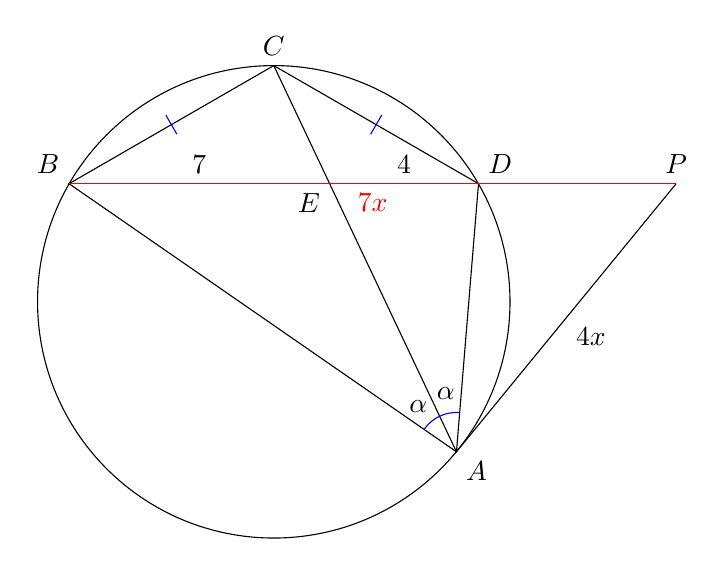
\begin{tikzpicture}[scale=0.5]
% define center O
\coordinate (O) at (0,0);
% draw circle with center O and radius 6
\draw (O) circle [radius=6];
% define points A, B, C, D, and E
\coordinate[label=below right:$A$] (A) at (4.64,-3.81);
\coordinate[label=above left:$B$] (B) at (-5.2,3);
\coordinate[label=above:$C$] (C) at (0,6);
\coordinate[label=above right:$D$] (D) at (5.2,3);
\coordinate[label=below left:$E$] (E) at (1.4181818,3);
\coordinate[label=above:$P$] (P) at (10.22,3);
\draw (B) -- (C) -- (D) -- (A) -- cycle;
\draw (C) -- (A);
\draw[red] (B) -- (P);

% length label
\node[red, below] at ($(B)!0.5!(P)$) {$7x$};
\node[above] at ($(B)!0.5!(E)$) {7};
\node[above] at ($(E)!0.5!(D)$) {4};
\node[below right] at ($(A)!0.5!(P)$) {$4x$};
\draw (P) -- (A);

%same angle
\pic[draw=blue, "$\alpha$", angle eccentricity=1.5] {angle = D--A--C};
\pic[draw=blue, "$\alpha$",  angle eccentricity=1.5] {angle = C--A--B};

\tkzMarkSegment[color=blue,pos=.5,mark=|](D,C) \tkzMarkSegment[color=blue,pos=.5,mark=|](B,C) 
\end{tikzpicture}
\end{center}
Sekarang, dari Alternate Segment Theorem, $\angle PAD = \angle ABP$. Karena diketahui juga $\angle DPA = \angle BPA$ maka didapatkan $\triangle DPA \sim \triangle APB$. Oleh karena itu, kita punya
$$\frac{PA}{PB} = \frac{AD}{BA} = \frac{4}{7}.$$
Berarti dapat dimisalkan $PA=4x$ dan $PB=7x$. Berarti $PD=PB-BD=7x-11$. Dari sini dengan Power of a Point, kita punya
$$PD \cdot PB = PA^2 \implies (7x-11)(7x) = (4x)^2 \implies 33x^2 = 77x \implies x = \frac{7}{3}.$$
Dari fakta tersebut, $\frac{PD}{PB} = \frac{7x-11}{7x}=\frac{16}{49}$ yang menyebabkan $m=16$ dan $n=49$ sehingga $m+n=\boxed{65}$.
\end{solusi}

\begin{soalbaru}
Jika bilangan asli $x$ dan $y$ memenuhi
$$x(x-y)=6y-7,$$
nilai dari $x+y$ adalah \dots
\end{soalbaru}
\begin{jawaban}
69
\end{jawaban}
\begin{solusi}
Kita punya
\begin{align*}
x(x-y)&=6y-7\\
x^2-xy &= 6y - 7\\
4x^2 - 4xy &= 24y - 28\\
4x^2 - 4xy + y^2 &= (y^2 + 24y + 144) - 144 - 28\\
(2x-y)^2 &= (y+12)^2 - 172\\
(y+12)^2-(2x-y)^2 &= 172\\
((y+12)+(2x-y))((y+12)-(2x-y)) &= 172\\
(2x+12)(2y-2x+12) &= 172\\
2(x+6)2(y-x+6) &= 172\\
(x+6)(y-x+6) &= 43
\end{align*}
dikarenakan $x+6 \ge 1+6 > 1$ dan $43$ adalah bilangan prima, maka haruslah $x+6 = 43 \implies x = 37$ dan $y-x+6=1 \implies y-37+6=1 \implies y = 32$. Oleh karena itu $x+y = \boxed{69}$.
\end{solusi}

\begin{soalbaru}
Misalkan $a_1,a_2,a_3,\dots$ suatu barisan yang memenuhi persamaan
$$a_{n+2}-a_{n+1}+a_{n}=\dfrac{n+2}{6}$$
untuk setiap bilangan asli $n$. Jika $a_1=3$ dan $a_2=4$, tentukan nilai dari $a_{2023}$.
\end{soalbaru}
\begin{jawaban}
337
\end{jawaban}
\begin{solusi}
Perhatikan bahwa untuk semua bilangan asli $n$ berlaku
\begin{align*}
(a_{n+3}-a_{n+2}+a_{n+1})+(a_{n+2}-a_{n+1}+a_{n})&=\dfrac{(n+1)+2}{6}+\dfrac{n+2}{6}\\
a_{n+3}+a_{n} &= \dfrac{2n+5}{6}
\end{align*}
berarti
\begin{align*}
(a_{2023}+a_{2020})+\dots+(a_7+a_4)+a_1 &= a_{2023}+(a_{2020}+a_{2017})+\dots+(a_4+a_1) \\
\dfrac{2(2020)+5}{6}+\dots+\dfrac{2(4)+5}{6} + a_1 &= a_{2023}+\dfrac{2(2017)+5}{6}+\dots+\dfrac{2(1)+5}{6}\\
\dfrac{2}{6}(2020+2014+\dots+4) + 337\left(\dfrac{5}{6}\right)+3&= a_{2023} + \dfrac{2}{6}(2017+2011+\dots+1) + 337\left(\dfrac{5}{6}\right)\\
\dfrac{2}{6}\left(\frac{337}{2}(2\cdot 4 + (337-1)6)\right) + 3 &= a_{2023} + \dfrac{2}{6}\left(\frac{337}{2}(2\cdot 1 + (337-1)6)\right) \\
\dfrac{2}{6}\left(\frac{337}{2}\cdot 2\cdot 4\right)-\dfrac{2}{6}\left(\frac{337}{2}\cdot 2\cdot 1\right)+3 &= a_{2023}\\
a_{2023} &= \boxed{337}.
\end{align*}
\end{solusi}

\begin{soalbaru}
Diberikan himpunan $S = \{a,b,c,d,e,f\}$. Akan dipilih dua subhimpunan dari $S$ yang gabungannya adalah $S$. Subhimpunan yang dipilih tidak harus berbeda. Urutan dari subhimpunan tidak diperhatikan. Banyak cara melakukan pemilihan adalah \dots
\end{soalbaru}
\begin{jawaban}
365
\end{jawaban}
\begin{solusi}
Misalkan ditinjau dua subhimpunan $X,Y$ dari $S$ dengan $X \cup Y = S$. Perhatikan bahwa setiap anggota $s \in S$ punya tiga keadaan berbeda yang saling lepas: 
\begin{enumerate}[1)]
\item $s \in X \backslash Y$,
\item $s \in Y \backslash X$, atau
\item $s \in  X \cap Y$. 
\end{enumerate}
Karena $|S| = 6$ berarti ada total $3^6 = 729$ cara. Perhatikan bahwa karena pembentukan $X$ dan $Y$ urutannya tak diperhatikan (yang berarti solusi $(X,Y)=(Y,X)$) maka saat $X \neq Y$, solusi $(X,Y)$ terhitung dua kali (sehingga hasil tadi dapat dibagi dua untuk mendapatkan salah satu solusi $(X,Y)$ untuk menghindari overcounting). Selanjutnya jika $X=Y$, maka $X=Y=S$ sehingga kemungkinan ini hanya dihitung satu kali (sehingga hasil di awal di kurang 1 sebelum dibagi 2 karena kasus ini tak termasuk yang overcounting). Oleh karena itu, dengan konsep simetri, maka banyaknya cara melakukan pemilihan subhimpunan tersebut adalah
$$\dfrac{3^6-1}{2}+1 = \boxed{365}$$
\end{solusi}

\begin{soalbaru}
Diberikan lingkaran $\Omega$ dan $AB$ merupakan tali busur dari $\Omega$. Lingkaran $\omega_1$ menyinggung $\Omega$ secara internal dan menyinggung $AB$ pada titik tengahnya. Lingkaran $\omega_2$ menyinggung $\Omega$ secara internal dan $\omega_1$ secara eksternal serta menyinggung $AB$. Jika jari-jari dari $\omega_1$ adalah 40 dan jari-jari dari $\omega_2$ adalah 8, tentukan panjang dari $AB$.
\begin{center}
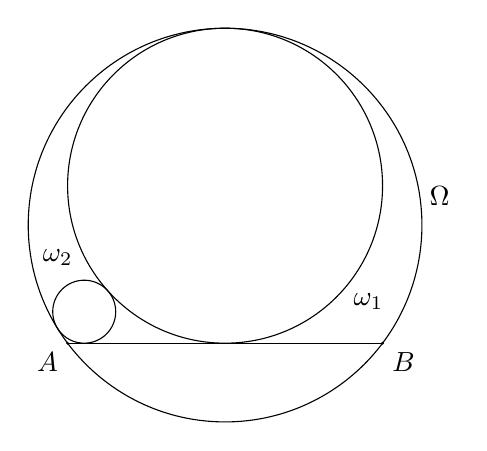
\begin{tikzpicture}[scale=0.5]
% draw circles
\coordinate (O) at (0,0);
\draw (O) circle [radius=5cm] node[label={$\Omega$}, right=2.6cm] {};
\coordinate (C) at (0,1);
\draw (C) circle [radius=4cm] node[label={$\omega_1$}, below right=2.4cm] {};
\coordinate (D) at (-3.57771, -2.2);
\draw (D) circle [radius=0.8cm] node[label={$\omega_2$}, above left=0.3cm] {};
% segment AB
\coordinate[label=below left:$A$] (A) at (-4,-3);
\fill (A) circle (0.04cm);
\coordinate[label=below right:$B$] (B) at (4,-3);
\fill (B) circle (0.04cm);
% segment
\draw (A) -- (B);
\end{tikzpicture}
\end{center}
\end{soalbaru}
\begin{jawaban}
80
\end{jawaban}

\begin{solusi}
Definisikan $O,C,D$ berturut-turut sebagai pusat lingkaran $\Omega, \omega_1, \omega_2$, lalu $K,M,F$ berturut-turut sebagai titik singgung $\omega_1$ dengan $\Omega, AB, \omega_2$. Selanjutnya misalkan $E,N$ berturut-turut sebagai titik singgung $\omega_2$ dengan $\Omega, AB$. Terakhir misalkan $KM$ memotong $\Omega$ kedua kalinya di $L$ dan misalkan $P$ pada $KL$ sedemikian sehingga $PM=DN$.
\begin{center}
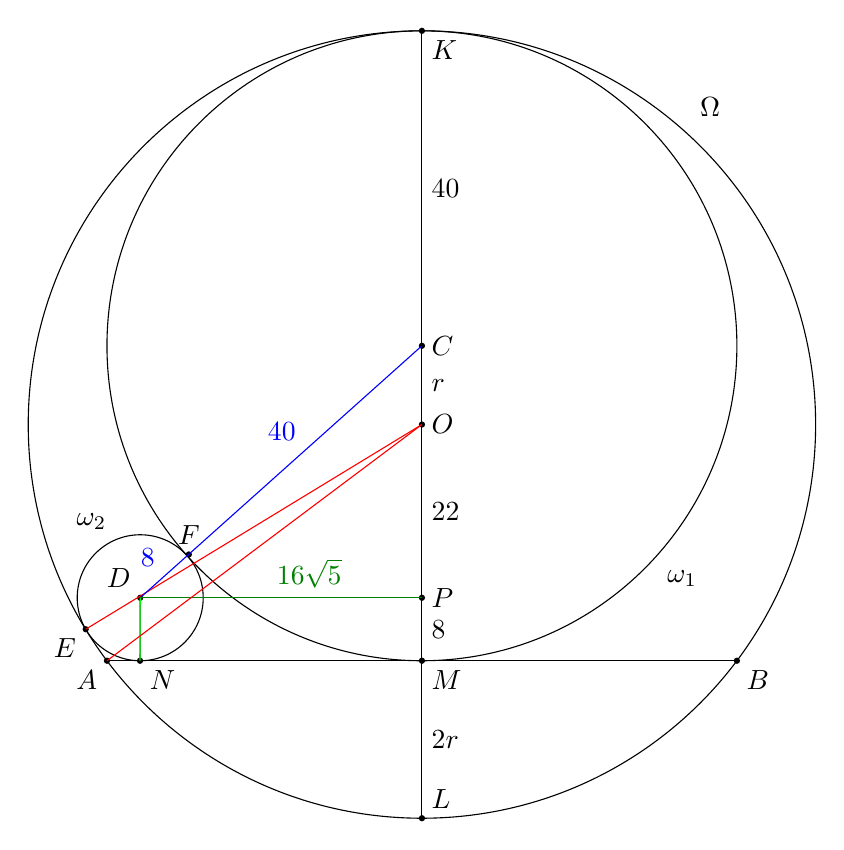
\begin{tikzpicture}
% draw circles
\coordinate[label=right:$O$] (O) at (0,0);
\draw (O) circle [radius=5cm] node[label={$\Omega$}, above right=5cm] {};
\fill (O) circle (0.04cm);
\coordinate[label=right:$C$] (C) at (0,1);
\draw (C) circle [radius=4cm] node[label={$\omega_1$}, below right=4.5cm] {};
\fill (C) circle (0.04cm);
\coordinate[label=above left:$D$] (D) at (-3.57771, -2.2);
\draw (D) circle [radius=0.8cm] node[label={$\omega_2$}, above left=0.7cm] {};
\fill (D) circle (0.04cm);
% segment AB
\coordinate[label=below left:$A$] (A) at (-4,-3);
\fill (A) circle (0.04cm);
\coordinate[label=below right:$B$] (B) at (4,-3);
\fill (B) circle (0.04cm);
\coordinate[label=below left:$E$] (E) at (-4.27,-2.6);
\fill (E) circle (0.04cm);
% tangent
\coordinate[label=above:$F$] (F) at (-2.96,-1.65);
\fill (F) circle (0.04cm);
\coordinate[label=below right:$M$] (M) at (0,-3);
\fill (M) circle (0.04cm);
\coordinate[label=below right:$N$] (N) at (-3.58,-3);
\fill (N) circle (0.04cm);
\coordinate[label=below right:$K$] (K) at (0,5);
\fill (K) circle (0.04cm);
\coordinate[label=above right:$L$] (L) at (0,-5);
\fill (L) circle (0.04cm);
\coordinate[label=right:$P$] (P) at (0,-2.2);
\fill (P) circle (0.04cm);
% segment
\draw (A) -- (B);
\draw (N) -- (D);
\draw[red] (E) -- (O);
\draw (K) -- (L);
\draw[blue] (C) -- (D);
\draw[green] (D) -- (N);
\draw[officegreen] (D) -- (P);
\draw[red] (O) -- (A);
% label length
\node at ($(K)!0.5!(C)$) [right] {40};
\node at ($(C)!0.5!(O)$) [right] {$r$};
\node at ($(O)!0.5!(P)$) [right] {22};
\node at ($(P)!0.5!(M)$) [right] {8};
\node at ($(M)!0.5!(L)$) [right] {$2r$};
\node at ($(C)!0.5!(F)$) [above left, blue] {40};
\node at ($(F)!0.5!(D)$) [above left, blue] {8};
\node at ($(D)!0.6!(P)$) [above, officegreen] {$16\sqrt{5}$};
\end{tikzpicture}
\end{center}
Misalkan $CO = r$. Berarti panjang jari-jari $\Omega$ adalah $KO =  40+r$. Perhatikan bahwa $CD = CF+Fd= 40+8=48$, $OD = OE-DE = (40+r)-8=32+r$, $CP = CM - PM = 40 - 8 = 32$, dan $OP = CP - CO = 32-r$. Oleh karena itu, dengan Pythagoras kita punya
\begin{align*}
DP^2 = CD^2 - CP^2 = 48^2 - 32^2 = 1280 \implies DP = 16\sqrt{5}
\end{align*}
dan
\begin{align*}
OD^2 - OP^2 &= DP^2\\
(32+r)^2 - (32-r)^2 &= 1280\\
(32^2+64r+r^2)-(32^2-64r+r^2) &= 1280\\
128r &= 1280\\
r &= 10.
\end{align*}
Itu berarti $OA=40+r=50$ dan $OM = CM - CO = 40-r=30$ sehingga $AM^2 = AO^2-OM^2 = 50^2 - 30^2 = 40^2 \implies AM = 40$. Sehingga, karena $M$ titik tengah $AB$ maka didapat $AB = 2 \cdot AM = \boxed{80}$.
\end{solusi}

\begin{soalbaru}
Misal, $N = 2^a \cdot 3^b$ dengan $a, b$ bilangan asli. Jika hasil kali semua faktor positif dari $N$ adalah $24^{60}$, maka nilai $ab$ adalah \dots
\end{soalbaru}
\begin{jawaban}
27
\end{jawaban}
\begin{solusi}
Perhatikan bahwa faktor-faktor dari $N$ berbentuk $2^i \cdot 3^j$ dimana $i=0,1,\dots,a$ dan $j=0,1,\dots,b$. Berarti hasil kali semua faktor positif dari $N$ dapat dinyatakan dengan
\begin{align*}
\prod_{i=0}^{a} \prod_{j=0}^{b} 2^i \cdot 3^j &= \prod_{i=0}^{a}  (2^i)^{b+1} \cdot 3^{0+1+\dots+b}\\
24^{60} &= \prod_{i=0}^{a}  (2^{b+1})^i \cdot 3^{\frac{b(b+1)}{2}}\\
(2^3\cdot 3)^{60} &= (2^{b+1})^{0+1+\dots+a} \cdot (3^{\frac{b(b+1)}{2}})^{a+1}\\
(2^3)^{60}\cdot3^{60} &= (2^{b+1})^{\frac{a(a+1)}{2}} \cdot (3^{\frac{b(b+1)}{2}})^{a+1}\\
2^{180}\cdot 3^{60} &= 2^{\frac{a(a+1)(b+1)}{2}} \cdot 3^{\frac{b(b+1)(a+1)}{2}}
\end{align*}
sehingga dengan membandingkan pangkat di kedua ruas didapat $\frac{a(a+1)(b+1)}{2}=180$ dan $\frac{b(b+1)(a+1)}{2}=60$. Berarti
$$\dfrac{a}{b}=\dfrac{\frac{a(a+1)(b+1)}{2}}{\frac{b(b+1)(a+1)}{2}}=\dfrac{180}{60}=3 \implies a = 3b.$$
Ini menyebabkan
$$60=\frac{b(b+1)(a+1)}{2}=\frac{b(b+1)(3b+1)}{2} \implies 3b^3+4b^2+b-120=0 \implies b=3 \implies a = 9.$$
Sehingga diperoleh $ab = 3 \cdot 9 = \boxed{27}$.
\end{solusi}

\begin{soalbaru}
Nilai minimum dari
$$\dfrac{(x+y)^2}{\sqrt{x^2-9}+\sqrt{y^2-16}}$$
adalah \dots
\end{soalbaru}
\begin{jawaban}
14
\end{jawaban}
\begin{solusi}
\textbf{Asumsi 1: $x$ dan $y$ real.} Karena $(x+y)^2$,$\sqrt{x^2-9}$, dan $\sqrt{y^2-16}$ nonnegatif, maka dengan memilih $x=-y$ diperoleh ekspresi di soal bernilai 0. Sehingga didapat nilai minimumnya adalah 0.

\textbf{Asumsi 2: $x$ dan $y$ real positif.} Misalkan $a = \sqrt{x^2-9}$ dan $b = \sqrt{y^2-16}$. Kita punya $x^2 = a^2 + 9$ dan $y^2 = b^2 + 16$. Dengan ketaksamaan Cauchy-Schwarz diperoleh
$$(xy)^2 = (a^2+9)(b^2+16) = (a^2+3^2)(b^2+4^2) \ge (ab+3\cdot 4)^2 = (ab+12)^2 $$
atau $xy \ge ab+12$. Selanjutnya dengan menggunakan ketaksamaan AM-GM dan ketaksamaan yang didapat sebelumnya, ekspresi di soal akan menjadi
\begin{align*}
\dfrac{x^2+y^2+2xy}{\sqrt{x^2-9}+\sqrt{y^2-16}}&=\dfrac{(a^2+9)+(b^2+16)+2xy}{a+b}\\
&=\dfrac{a^2+b^2+2ab}{a+b}+\dfrac{2xy-2ab+25}{a+b}\\
&=\dfrac{(a+b)^2}{a+b}+\dfrac{2xy-2ab+25}{a+b}\\
&=(a+b)+\dfrac{2xy-2ab+25}{a+b}\\
&\ge 2\sqrt{(a+b)\left(\dfrac{2xy-2ab+25}{a+b}\right)} \quad (AM-GM)\\
&= 2\sqrt{2xy-2ab+25}\\
&\ge 2\sqrt{2(ab+12)-2ab+25} \quad (xy \ge ab+12)\\
&= 2\sqrt{49}\\
&= \boxed{14}
\end{align*}
dengan kesamaan terjadi saat
\end{solusi}

\begin{soalbaru}
Diberikan 100 titik seperti pada gambar berikut (jarak tiap titik sama)
\begin{center}
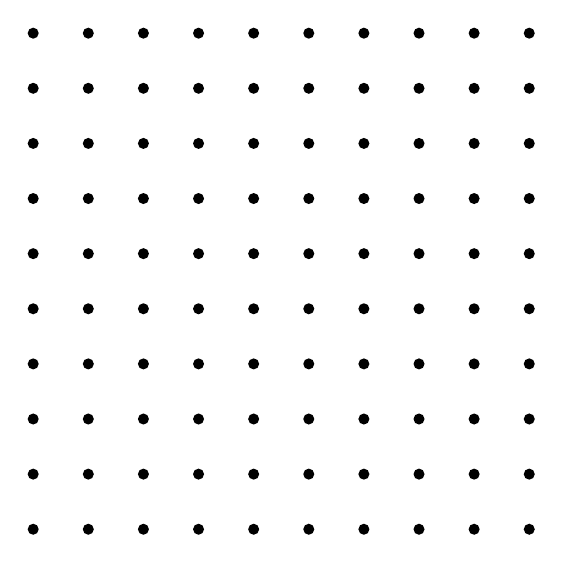
\begin{tikzpicture}[scale=0.7]
    \draw[step=1cm,draw opacity=0.0] (0,0) grid (9,9);
    \foreach \x in {0,1,2,...,9}
        \foreach \y in {0,1,2,...,9}
            \fill (\x,\y) circle (0.1cm);
\end{tikzpicture}
\end{center}
Banyak persegi yang semua titik sudutnya adalah 4 titik diantara titik-titik pada gambar tersebut adalah \dots
\end{soalbaru}
\begin{jawaban}
825
\end{jawaban}
\begin{solusi}
Tinjau koordinat kartesius dengan ujung paling kiri bawah adalah $(0,0)$ dan ujung paling kanan atas adalah $(9,9)$. Sebut daerah 100 titik tersebut dengan "kotak". Misalkan persegi yang akan dihitung banyaknya adalah persegi $ABCD$ dimana $A(x,y)$, $B(x+a, y+b)$, $C(x+a+b,y+b-a)$, dan $D(x+b, y-a)$ dengan $x,y,a,b$ suatu bilangan bulat non-negatif.
\begin{center}
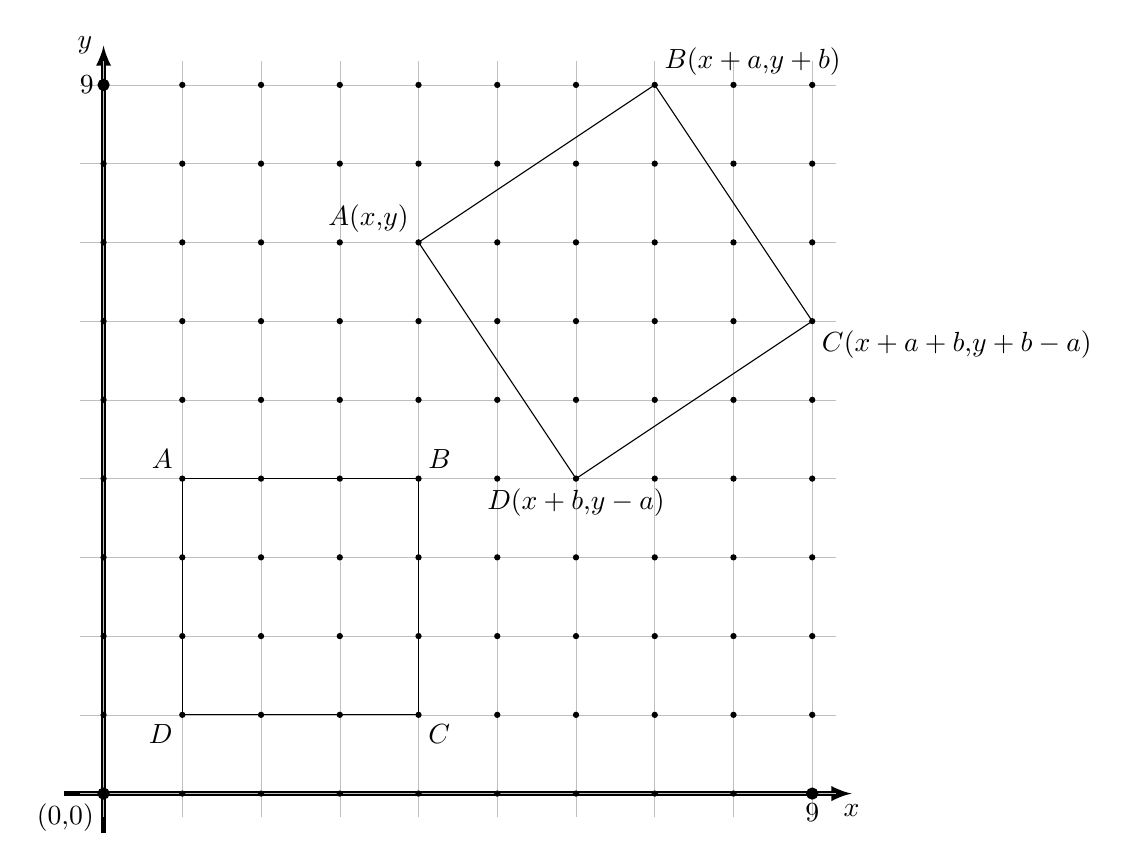
\begin{tikzpicture}
% x-axis
\draw[-latex, line width=1.5pt] (-0.5,0) -- (9.5,0) node[below] {$x$};
% y-axis
\draw[-latex, line width=1.5pt] (0,-0.5) -- (0,9.5) node[left] {$y$};
% grid
\draw[step=1cm,gray!50,very thin] (-0.3,-0.3) grid (9.3,9.3);

\foreach \x in {0,1,2,...,9}
        \foreach \y in {0,1,2,...,9}
            \fill (\x,\y) circle (0.04cm);
\filldraw (0,0) circle (2pt) node[below left] {$(0\text{,}0)$};
\filldraw (9,0) circle (2pt) node[below] {$9$};
\filldraw (0,9) circle (2pt) node[left] {$9$};
\coordinate[label=above left:$A$] (A) at (1,4);
\coordinate[label=above right:$B$] (B) at (4,4);
\coordinate[label=below right:$C$] (C) at (4,1);
\coordinate[label=below left:$D$] (D) at (1,1);
\draw (A) -- (B) -- (C) -- (D) -- cycle;

\coordinate[label=above left:$A(x\text{,}y)$] (E) at (4,7);
\coordinate[label=above right:$B(x+a\text{,}y+b)$] (F) at (7,9);
\coordinate[label=below right:$C(x+a+b\text{,}y+b-a)$] (G) at (9,6);
\coordinate[label=below:$D(x+b\text{,}y-a)$] (H) at (6,4);
\draw (E) -- (F) -- (G) -- (H) -- cycle;
\end{tikzpicture}
\end{center}
 Karena urutan titik sudut tidak diperhatikan atau persegi yang didapat dari rotasi $90^\circ$ persegi lain dianggap persegi yang sama, maka tanpa mengurangi keumuman, pilih $a \ge 1,b \ge 0$ agar persegi yang terbentuk selalu memiliki panjang sisi lebih dari sama dengan 1, $A$ selalu berada di kiri $B$, dan $D$ tidak pernah di kiri $A$. Oleh karena itu kita punya batasan $0 \le x$; $y+b \le 9$; $x+a+b \le 9$; dan $0 \le y-a$; berturut-turut agar titik $A$, $B$, $C$, dan $D$ tidak berada di luar kotak. Berarti jika batasan tersebut digabungkan, kita punya
 $$
 \begin{cases}
 1 &\le a\\
 0 &\le b\\ 
 0 &\le x \le 9-(a+b)\\
 0 &\le y-a \le 9-(a+b).
 \end{cases}
 $$
 Untuk setiap $a$ dan $b$ yang memenuhi, banyaknya $x$ dan $y$ yang memenuhi masing-masing adalah $9-(a+b)+1 = 10-a-b$ yaitu $x,y = 0,1,\dots,9-(a+b)$. Berarti untuk setiap pasang $(a,b)$ yang memenuhi banyaknya persegi yang dapat terbentuk adalah $(10-a-b)^2$  Oleh karena itu kita tinggal mengobservasi seluruh kemungkinan $a+b$ yang memenuhi.
 \begin{itemize}
 \item Untuk $a+b=1$, pasangan $(a,b)$ yang memenuhi ada 1 yaitu $(1,0)$ sehingga banyak persegi yang terbentuk adalah $1 \times (10-1)^2 = 81$.
 \item Untuk $a+b=2$, pasangan $(a,b)$ yang memenuhi ada 2 yaitu $(2,0),(1,1)$ sehingga banyak persegi yang terbentuk adalah $2 \times (10-2)^2 = 128$.
 \item Untuk $a+b=3$, pasangan $(a,b)$ yang memenuhi ada 3 yaitu $(3,0),(2,1),(1,2)$ sehingga banyak persegi yang terbentuk adalah $3 \times (10-3)^2 = 147$.
 \item Untuk $a+b=4$, pasangan $(a,b)$ yang memenuhi ada 4 yaitu $(4,0),\dots,(1,3)$ sehingga banyak persegi yang terbentuk adalah $4 \times (10-4)^2 = 144$.
 \item Untuk $a+b=5$, pasangan $(a,b)$ yang memenuhi ada 5 yaitu $(5,0),\dots,(1,4)$ sehingga banyak persegi yang terbentuk adalah $5 \times (10-5)^2 = 125$.
 \item Untuk $a+b=6$, pasangan $(a,b)$ yang memenuhi ada 6 yaitu $(6,0),\dots,(1,5)$ sehingga banyak persegi yang terbentuk adalah $6 \times (10-6)^2 = 96$.
 \item Untuk $a+b=7$, pasangan $(a,b)$ yang memenuhi ada 7 yaitu $(7,0),\dots,(1,6)$ sehingga banyak persegi yang terbentuk adalah $7 \times (10-7)^2 = 63$.
 \item Untuk $a+b=8$, pasangan $(a,b)$ yang memenuhi ada 8 yaitu $(8,0),\dots,(1,7)$ sehingga banyak persegi yang terbentuk adalah $8 \times (10-8)^2 = 32$.
 \item Untuk $a+b=9$, pasangan $(a,b)$ yang memenuhi ada 9 yaitu $(9,0),\dots,(1,8)$ sehingga banyak persegi yang terbentuk adalah $9 \times (10-9)^2 = 9$.
 \end{itemize}
 Berarti didapat total persegi yang memenuhi adalah $81+128+147+144+125+96+63+32+9=\boxed{825}$.
\end{solusi}

\begin{soalbaru}
Diberikan segitiga $ABC$. Misal titik $D,E,F$ terletak pada sisi $BC,CA,AB$ sehingga $AD,BE,CF$ berpotongan di satu titik. Diketahui bahwa $\angle EDF = 56^\circ$. Jika $\angle ADB = 90^\circ$ dan $AF=FB$, maka besar sudut $\angle ABC$ adalah \dots
\end{soalbaru}
\begin{jawaban}
$62^\circ$
\end{jawaban}
\begin{solusi} Perhatikan karena $AF=FB$ dan $\angle ADB = 90^\circ$, maka $DF=FA$. Berarti jika dimisalkan $\angle FDA = x$ maka $\angle FAD = \angle FDA = x$. 
\begin{center}
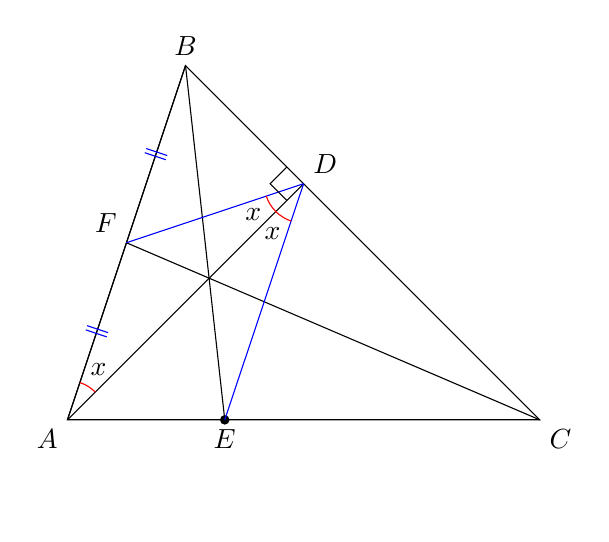
\begin{tikzpicture}[scale=1.5]
    \coordinate[label=below left:$A$] (A) at (0,0);
    \coordinate[label=below right:$C$] (C) at (4,0);
    \coordinate[label=above:$B$] (B) at (1,3);
    \draw (A) -- (B) -- (C) -- cycle;
    \coordinate[label=above left:$F$] (F) at ($(A)!0.5!(B)$);
    \draw (A) -- (F) -- (B);
    \coordinate[label=above right:$D$] (D) at ($(B)!(A)!(C)$);
    \draw[name path=A--D] (A) -- (D);
    \draw[name path=C--F] (C) -- (F);
	\path [name intersections={of=A--D and C--F,by=T}];
    \draw[name path=B--T, opacity=0] (B) -- ($(T)!-2cm!(B)$);
    \draw[name path=C--A] (C) -- (A);	
	\path [name intersections={of=B--T and C--A,by=E}];
	\filldraw (E) circle (1pt) node[below] {$E$};
	\draw (B) -- (T) -- (E);
    \draw[blue] (F) -- (D);
    \draw[blue] (E) -- (D);
    
    % angle
    \siku{A}{D}{B}
    \pic[draw=red, "$x$", angle eccentricity=1.5] {angle = D--A--F};
    \pic[draw=red, "$x$", angle eccentricity=1.5] {angle = F--D--A};
    \pic[draw=red, "$x$", angle eccentricity=1.5] {angle = A--D--E};
    
    \tkzMarkSegment[color=blue,pos=.5,mark=||](B,F) 
    \tkzMarkSegment[color=blue,pos=.5,mark=||](F,A) 
\end{tikzpicture}
\end{center}
\vspace{-1cm}
Sekarang perhatikan karena $AD,BE,CF$ bertemu di satu titik dan $\frac{BF}{FA}=1$ maka dengan Teorema Ceva
$$\frac{BF}{FA}\cdot \frac{AE}{EC} \cdot \frac{CD}{DB} = 1 \implies \frac{AE}{EC} = \frac{DB}{CD} \implies DE \parallel BA.$$
Dari sini, karena $DE \parallel BA$ maka $\angle EDA = \angle DAF = x$. Hal tersebut mengakibatkan $56^\circ =\angle EDF = 2x \implies x = 28^\circ$. Berarti kita akan mendapat $\angle ABC = 90^\circ - \angle BAD = 90^\circ - x = \boxed{62^\circ}.$
\end{solusi}

\begin{soalbaru}
Misal $p$ dan $n$ adalah dua bilangan asli dengan $p$ prima sehingga $p$ membagi $n^2+4$ dan $n$ membagi $p^2+4$. Jika $p<200$, nilai terbesar yang mungkin dari $n$ adalah \dots
\end{soalbaru}
\begin{jawaban}
169
\end{jawaban}
\begin{solusi}
Perhatikan bahwa $(p,n) = (2,2)$ memenuhi. Jika $p = 3$ maka $n \mid 3^2+4 = 13$ sehingga $n=1,13$. Ini menyebabkan $3 \mid 1^2+4$ atau $3 \mid 13^2 + 4$ yang keduanya merupakan kontradiksi. 

Oleh karena itu asumsikan $p> 3$ atau $p \ge 5$ dan $n > 1$. Tinjau $p | n^2+4$ dan $n | p^2+4$ sehingga
$$pn \mid (n^2+4)(p^2+4) \implies pn | (pn)^2 + 4(p^2 + n^2 + 4) \implies pn | p^2+n^2+4.$$
maka $p^2+n^2+4 = kpn$ untuk suatu $k\in \mathbb{N}$. Tinjau persamaan diophantine $x^2+y^2+4=kxy$ dengan solusi pasangan bilangan asli $(x,y)$. Observasi bahwa jika $(x,y)$ solusi, maka berdasarkan kesimetrian, $(y,x)$ juga solusi. 

Sekarang, tinjau bahwa persamaan tersebut setara dengan
$$x^2 -ky \cdot x + (y^2+4)=0$$
yang merupakan persamaan kuadrat dalam $x$. Untuk mencari solusi seprti yang diminta soal, akan dicari solusi $(x,y)$ dimana setidaknya salah satu dari $x,y < 200$ dan bilangan prima. Dari teorema Vieta, jika $x_1$ dan $x_2$ adalah akar-akar persamaan tersebut, kita punya $x_1 + x_2 = ky$ dan $x_1x_2 = y^2+4$. Jika $x_1, y \in \mathbb{N}$ maka $x_2 = ky - x_1 \in \mathbb{Z}$. Namun, karena $x_1x_2 = y^2 + 4 > 0$ maka $x_2 \in \mathbb{N}$. Berarti jika $(x_1, y)$ solusi, maka $(y, x_2) = (y, \frac{y^2+4}{x_1})$ juga solusi. Akan ditinjau proses mendapatkan pasangan-pasangan solusi tersebut. Notasikan dengan panah seperti pada ilustrasi berikut
$$(x_1, y) \rightarrow (y, \tfrac{y^2+4}{x_1}) \rightarrow \cdots .$$
Perhatikan bahwa $(x,y)=(1,5)$ merupakan solusi. Oleh karena itu kita punya
$$(1,5) \rightarrow (5,29) \rightarrow (29, 169) \rightarrow (169, 985) \rightarrow (985, 5741) \rightarrow \cdots .$$
Sadari bahwa hanya $(1,5),(5,29),(29,169)$ yang minimal salah satu bilangannya kurang dari 200 dan prima. Oleh karena itu, solusi yang menghasilkan $n$ terbesar pada ekspresi di soal adalah $(p,n) = (29, 169)$ sehingga $n$ terbesarnya adalah $\boxed{169}$.
\end{solusi}

\end{document}
